\documentclass[a4paper]{article}
\usepackage[margin=1in]{geometry}
\usepackage[utf8]{inputenc}
\usepackage[english]{babel}
%\usepackage{graphicx}
\usepackage{amssymb}
\usepackage{amsmath}
\usepackage{amsthm}
%\usepackage{listings} % Darstellen von Codebeispielen
\usepackage{titlesec}
%\usepackage{chngcntr}
\usepackage{mathtools}
\usepackage{algorithm}
\usepackage{algpseudocode}
\usepackage[normalem]{ulem}
%\usepackage{float}
%\usepackage{cite}
\counterwithin{figure}{section}
\newcommand{\sectionbreak}{\clearpage}
\usepackage[round]{natbib}
\usepackage{float}
\usepackage{svg}
\usepackage{fancyhdr}
\pagestyle{fancy}
\usepackage[hidelinks]{hyperref}
\usepackage{todonotes}

\mathtoolsset{showonlyrefs}

\DeclareMathOperator{\argmax}{argmax}
\DeclareMathOperator{\argmin}{argmin}
%\DeclareMathOperator{\next}{next}
\DeclareMathOperator{\prev}{prev}
\DeclareMathOperator{\on}{on}
\DeclareMathOperator{\off}{off}
\DeclareMathOperator{\idle}{idle}
\DeclareMathOperator{\act}{active}
\DeclareMathOperator{\costs}{costs}
\DeclareMathOperator{\adjacent}{adjacent}
\DeclareMathOperator{\neighboring}{neighboring}
\DeclareMathOperator{\true}{true}
\DeclareMathOperator{\false}{false}
\DeclareMathOperator{\ifop}{if}
\DeclareMathOperator{\elseop}{otherwise}
\DeclareMathOperator{\OPT}{OPT}
\DeclareMathOperator{\PLTR}{PLTR}
\DeclareMathOperator{\fv}{fv}
\DeclareMathOperator{\uv}{uv}
\DeclareMathOperator{\pv}{pv}
\DeclareMathOperator{\vol}{v}
\DeclareMathOperator{\opdef}{def}
\DeclareMathOperator{\exc}{exc}
\DeclareMathOperator{\keepidle}{keepIdle}
\DeclareMathOperator{\keepactive}{keepActive}
\DeclareMathOperator{\rank}{rank}
\DeclareMathOperator{\crit}{crit}


\newtheorem{theorem}{Theorem}
\newtheorem{lemma}[theorem]{Lemma}
\newtheorem{definition}[theorem]{Definition}
%\newtheorem*{remark}{Remark}


\title{Greedy Energy-Efficient Scheduling Algorithms for Processor Systems}
%\author{Gunther Bidlingmaier}
%\date{15.11.2020}

\begin{document}

\selectlanguage{english}
%\frontmatter{}
%\input{pages/acknowledgements}

%\maketitle
\begin{abstract}
  We study a particular scheduling setting in which a set of $n$ jobs with individual release times and deadlines has to be scheduled across $m$ homogeneous processors while minimizing the consumed energy.
  Idle processors can be turned off so as to save energy, while turning them on requires a fixed amount of energy.
  For the special case of a single processor, the greedy algorithm Left-to-Right guarantees an approximation factor of $2$.
  We generalize this simple greedy policy to the case of multiple processors and show that the energy costs are still bounded by $2 \OPT + P$.
  Our algorithm has a running time of $(n + m) \log(d^*) F$ where $d^*$ is the largest deadline and $F$ the costs of a maximum flow calculation for checking feasibility of an instance.
\end{abstract}

\tableofcontents

\section{Algorithm}
\todo{Formal Problem definition, notation}
\todo{Formulate and format keepactive, keepidle nicer.}
\todo{Properly define scheduling problem with lower and upper bounds $l_t, m_t$.}
\todo{Precisely relate $l_t, m_t$ returned by Algorithm to assignment of jobs to processors, time slots.}
\begin{algorithm}[H]
\caption{Parallel Left-to-Right}\label{alg:RECLTR}
\begin{algorithmic}
  \State{} $m_t \gets m$
  \State{} $l_t \gets 0$
  \For{$k \gets m$ \textrm{to} $1$}
    \State{$t\gets0$}
    \While{$t < d^*$}
      \State{$t \gets $\Call{KeepIdle}{k, t}}
      \State{$t \gets $\Call{KeepActive}{k, t}}
    \EndWhile{}
  \EndFor{}

  \Function{KeepIdle}{k, t}
    \State{search for maximal $t' \geq t$ s.t.\
    exists feasible schedule with $m_{t''} = k-1 \forall t'' \in [t, t')$}
    \State{$m_{t''} \gets k - 1 \forall t'' \in [t, t')$}
    \State{\Return{$t'$}}
  \EndFunction{}
  \Function{KeepActive}{k, t}
    \State{search for maximal $t' \geq t$ s.t.\
    exists feasible schedule with $l'_{t''} = \max\{k, l_{t''}\}k-1 \forall t'' \in [t, t')$}
    \State{$m_{t''} \gets k - 1 \forall t'' \in [t, t')$}
    \State{\Return{$t'$}}
  \EndFunction{}
  %\Function{IsFeasible}{\null}
  %  \State{$f^* \gets$ Max-Flow for current values of $m_t, l_t$}
  %  \State{\Return{$f^* == P$}}
  %\EndFunction{}
\end{algorithmic}
\end{algorithm}


\begin{figure}[H]
  \centering
  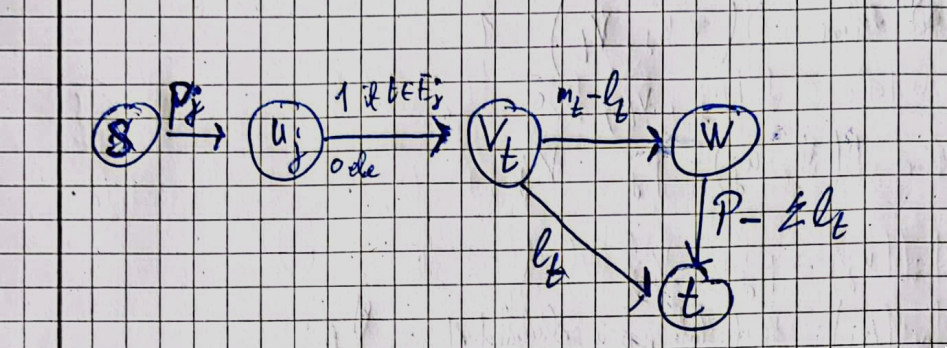
\includegraphics[width=\textwidth]{graphics/sketches/flow_network.png}
  \label{fig:flow}
  \caption{The Flow-Network for checking feasibility of a scheduling instance with lower and upper bounds $l_t$ and $m_t$ for the number of active processors at $t$.}
\end{figure}

\todo{Ambiguity of $t$ used for time slots and sink in flow-network: Use $\alpha$-$\omega$ flow}
\todo{Briefly define $c$ for edge capacities and cuts.}
\todo{Introduce notation for number of jobs scheduled at $t$?}

\begin{lemma}\label{lemma:flow_feasibility}
  There exists a feasible solution to a scheduling instance with lower and upper bounds $l_t, m_t$ if and only if the maximum $s$-$t$ flow in the corresponding flow network depicted in Figure~\ref{fig:flow} has value $P$.
\end{lemma}
\begin{proof}
  Let $f$ be a $s$-$t$ flow of value $|f| = P$.
  We construct a feasbile schedule from $f$ respecting the lower and upper bounds given by $l_t$ and $m_t$.
  For every $j \in J$ and  $t \in [0, d^*]$, if $f(u_j, v_t) = 1$, then schedule $j$ at slot $t$.
  Since $|f| = P$ and the capacity $c(\{s\}, V \setminus \{s\}) = P$, we have $f_{in}(u_j) = p_j$ for every $j \in J$.
  Hence $f_{out}(u_j) = \sum_{t \in E_j} f_{in}(v_t) = p_j$.
  Hence every job $j$ is scheduled in $p_j$ distinct time slots.

  The schedule respects the upper bounds $m_t$, since $c(v_t, w) + c(v_t, t) \leq m_t - l_t + l_t$ and for every $t$ at most $m_t$ jobs are scheduled at $t$. 

  The schedule respects the lower bounds $l_t$, since
  $c(V \setminus \{t\}, \{t\}) = P$ and hence
  $f(v_t, t) = l_t$ for every slot $t$.
  By flow conservation we then have $f_{in}(v_t) \geq l_t$ which implies that at least $l_t$ jobs are scheduled at every slot $t$.

  For the other direction consider a feasible schedule respecting the lower and upper bounds $l_t, m_t$.
  We construct a flow $f$ of value $P$ and show that it is maximal.

  If $j$ is scheduled at slot $t$ and hence $t \in E_j$,
  define $f(u_j, v_t) = 1$, otherwise $f(u_j, v_t) = 0$.
  Define $f(s, u_j) = p_j$ for every $j \in J$.
  Hence we have $f_{in}(u_j) = p_j$
  and $f_{out}(u_j)$ must be  $p_j$ since this corresponds to the number of distinct time slots in which $j$ is scheduled.
  Define $f(v_t, t) = l_t$ for every slot $t$.
  Define $f(v_t, w) = f_{in}(v_t) - l_t$.
  We have $f(v_t, w) \leq m_t - l_t$ since $f_{in}(v_t)$ corresponds to the number of jobs scheduled at $t$, which is at most $m_t$.
  We also have $f_{out}(v_t) = f_{in}(v_t) - l_t + l_t = f_{in}(v_t)$.

  Define $f(w, t) = P - \sum_t l_t$.
  Then $f_{in}(w) = \sum_t f_{in}(v_t) - l_t
  = \sum_t |\{j \in J \mid j~\text{scheduled at}~t\}| - \sum_t l_t$.
  Since the schedule is feasible, this corresponds to
  $f_{in}(w) = P - \sum_t l_t = f_{out}(w)$.

\end{proof}

\section{Structure of the PLTR-Schedule}
\subsection{Preliminary Definitions}
\todo{Use $T = [0, d^*]$ here?}
\begin{definition}
  For schedule $S$, we define the \emph{volume} $\vol_S(j, Q)$ of job $j \in J$ in a set $Q \subseteq [0, d^*]$ of time slots as the number of time slots of $Q$ for which $j$ is scheduled at by $S$.
\end{definition}
\begin{definition}
  We define the \emph{forced volume} $\fv(j, Q)$ of job $j \in J$ in a set $Q \subseteq [0, d^*]$ of time slots as the number of time slots of $Q$ for which $j$ has to be scheduled in every feasible schedule, i.e.
  \begin{align}
    \fv(j, Q) = \max\{0; p_j - |E_j \setminus Q|\}
  \end{align}
\end{definition}
\begin{definition}
  We define the \emph{unnecessary volume} $\uv_S(j, Q)$ of job $j \in J$ in a set $Q \subseteq [0, d^*]$ of time slots as the amount of volume which does not have to scheduled during $Q$, i.e.
  \begin{align}
    \uv_S(j, Q) = \vol_S(j, Q) - \fv(j,Q)\text{.}
  \end{align}
\end{definition}
\begin{definition}
  We define the \emph{possible volume} $\pv(j, Q)$ of job $j \in J$ in a set $Q \subseteq [0, d^*]$ of time slots as the maximum amount of volume which $j$ can be feasibly scheduled in $Q$, i.e.
  \begin{align}
    \pv(j, Q) = \min\{ p_j, |E_j \cap Q \} \text{.}
  \end{align}
\end{definition}
Since the corresponding schedule $S$ will usually be clear from context, we drop the subscript for the volume and the unnecessary volume.
We extend our volume definitions to sets $J' \subseteq J$ of jobs by summing over all $j \in J'$, i.e.
\begin{align}
  \vol(J', Q) = \sum_{j \in J'} \vol(j, Q)\text{.}
\end{align}
If the first parameter is dropped, we refer to the whole set $J$, i.e.\ $\vol(Q) = \vol(J, Q)$.
Clearly we have for every feasible schedule, every $Q, j$ that $\fv(j, Q) \leq \vol(j, Q) \leq \pv(j, Q)$.

\begin{definition}
  We define the \emph{density} $\phi(Q)$ for a set $Q \subseteq [0, d^*]$ as the average amount of processing volume which has to be completed in every slot of $Q$, i.e.
  $\phi(Q) = \fv(J, Q) / |Q|$.
  We also define $\widehat \phi(Q) = \max_{Q' \subseteq Q} \phi(Q')$.
\end{definition}
If $\widehat \phi(Q) > k - 1$, then clearly at least $k$ processors are required in some time slot $t \in Q$ for every feasible schedule.
\begin{definition}
  We define the \emph{deficiency} $\opdef(Q)$ of a set $Q \subseteq [0, d^*]$ of time slots as the difference between the amount of volume which has to be completed in $Q$ and the processing capacity available in $Q$, i.e. $\opdef(Q) = \fv(Q) - \sum_{t \in Q} m_t$.
\end{definition}
\begin{definition}
  We define the \emph{excess} $\exc(Q)$ of a set $Q \subseteq [0, d^*]$ of time slots as the difference between the processor utilization required in $Q$ and the amount of processing volume available in $Q$, i.e. $\exc(Q) = \sum_{t \in Q} l_t - \pv(Q)$.
\end{definition}
\subsection{Critical set of time slots}
\begin{lemma}\label{lemma:cut}
  For every $s$-$t$ cut $(S, \bar S)$ we have at least one of the following two lower bounds for the capacity $c(S)$ of the cut:
  $c(S) \geq P - \opdef(Q(S))$ or $c(S) \geq P - \exc(Q(\bar S))$, where $Q(S) \coloneqq \{ t \mid v_t \in S \}$.
\end{lemma}
\begin{proof}
  Let $(S, \bar S)$ be a $s$-$t$ cut, let $J(S) \coloneqq \{j \mid u_j \in S\}$.
  We consider 
  If $w \notin S$, consider the contribution of every node of $S$ to the capacity of the cut.
  \begin{itemize}
    \item Node $s$: $\sum_{j \in J(\bar S)} p_j$.
    \item Node $u_j$: $|\{v_t \in \bar S \mid t \in E_j\}| = | E_j \setminus Q(S) | \geq p_j - \fv(j, Q(S))$
    \item Node $v_t$: $l_t + m_t - l_t = m_t$
  \end{itemize}
  The inequality for node $u_j$ follows since $\fv(j, Q(S)) = \max \{0, p_j - |E_j \setminus Q(S)| \}$.
  In total, we can lower bound the capacity with 
  \begin{align}
    c(S) &\geq \sum_{j \in J(\bar S)} p_j + \sum_{j \in J(S)} p_j - \fv(j, Q(S)) + \sum_{t \in Q(S)} m_t
    \\ &= P - \fv(J(S), Q(S)) + \sum_{t \in Q(S)} m_t
    \\ &\geq P - \opdef(Q(S))\text{.}
  \end{align}
  If $w \in S$, again consider the contribution of every node of $S$ to the capacity of the cut.
  \begin{itemize}
    \item Node $s$: $\sum_{j \in J(\bar S)} p_j \geq \pv(J(\bar S), Q(\bar S))$.
    \item Node $u_j$: $| E_j \setminus Q(S) |
      = | E_j \cap Q(\bar S)| \geq \pv(j, Q(\bar S))$
    \item Node $v_t$: $l_t$
    \item Node $w$: $P - \sum_t l_t$
  \end{itemize}
  In total, we can lower bound the capacity with 
  \begin{align}
    c(S) &\geq P - \sum_{t \in Q(\bar S)} l_t + \pv(Q(\bar S))
    \\ &= P - \exc(Q(\bar S))
  \end{align}

\end{proof}

\begin{lemma}\label{lemma:feasibility}
  A scheduling instance with lower and upper bounds $l_t$ and $m_t$ is feasible if and only if $\opdef(Q) \leq 0$ and $\exc(Q) \leq 0$ for every $Q \subseteq [0, d^*]$.
\end{lemma}
\begin{proof}
  If $\opdef(Q) > 0$ for some $Q$, then some upper bounds $m_t$ cannot be met.
  If $\exc(Q) > 0$ for some $Q$, then some lower bound $l_t$ cannot be met.
  For the direction from right to left, consider an infeasible scheduling instance with lower and upper bounds.
  By Lemma~\ref{lemma:flow_feasibility} we have that the maximum flow $f$ for this instance has value $|f| < P$.
  Hence, there must be a $s$-$t$ cut $(S, \bar S)$ of capacity $c(S) < P$.
  Lemma~\ref{lemma:cut} now implies that $\opdef(Q(S)) > 0$ or $\exc(Q(\bar S)) > 0$.
\end{proof}
\begin{lemma}\label{lemma:critical}
  For every time slot $t \in [0, d^*]$ for which some processor $k \in [m]$ is activated in $S_{\PLTR}$, there exists a set $Q \subseteq [0, d^*]$ of time slots with $t \in Q, $
  \begin{align}
    \fv(Q) &= v(Q) \text{,}\\
    \vol(t') &\geq k-1 &~\text{for}~t' \in Q~\text{and}\\
    \vol(t') &\geq k &~\text{for}~t' \in Q~\text{with}~t' \geq t \text{.}
  \end{align}
\end{lemma}
\begin{proof}
  Suppose for contradiction there is some activation $t \in [0, d^*]$ of processor $k \in [m]$ and no such $Q$ exists for $t$.
  We show that $\PLTR$ would have extended the idle interval on processor $k$ which ends at $t$.
  Consider the step in $\PLTR$ when $t$ was the result of $\keepidle$ on processor $k$ and the corresponding lower and upper bounds $m_{t'}, l_{t'}$ for $t' \in [0, d^*]$ right after the calculation of $t$ and the corresponding update of the bounds by $\keepidle$.
  We modify the bounds by decreasing $m_t$ by $1$.
  Note that at this point $m_{t'} \geq k$ for every $t' > t$ and $m_{t'} \geq k - 1$ for every $t'$.
  
  Consider $Q \subseteq [0, d^*]$ s.t.\ $t \in Q$ and $\fv(Q) < \vol(Q)$.
  Before our modification we had $m_Q \coloneqq \sum_{t' \in Q} m_{t'} \geq \vol(Q) > \fv(Q)$.
  The inequality $m_Q \geq \vol(Q)$ here follows since the upper bounds $m_{t'}$ are monotonically decreasing during $\PLTR$.
  After our modification we still have $m_Q \geq \fv(Q)$.

  Consider $Q \subseteq [0, d^*]$ s.t.\ $t \in Q$ and $v(t') < k - 1$ for some $t'$.
  At the step in $\PLTR$ considered by us, we hence have $m_{t'} \geq k - 1 > v(t')$ and therefore before our decrement of $m_t$ we had $m_Q > \vol(Q) \geq \fv(Q)$ which implies $m_Q \geq \fv(Q)$ after the decrement of $m_t$.

  Finally, consider $Q \subseteq [0, d^*]$ s.t.\ $t \in Q$ and $v(t') < k$ for some $t' > t$.
  Again at the step in $\PLTR$ considered by us, we have $m_{t'} \geq k > v(t')$ which implies $m_Q \geq \fv(Q)$ after our decrement of $m_t$.
  
  If for $t$ no $Q$ exists as characterized in the proposition, $t$ cannot have been the result of $\keepidle$ at this step in $\PLTR$, which is a contradiction.
\end{proof}

\begin{definition}
  We call such $Q$ for activations $t$ of processor $k$ characterized by Lemma~\ref{lemma:critical} \emph{tight set $Q_t$ over activation $t$ of processor $k$}.
\end{definition}

\begin{definition}
  A \emph{critical set $C_t \subseteq [0, d^*]$ over an activation $t$} is the maximum of the set of tight sets $Q_t$ over activation $t$ in regard to the density $\phi$, i.e.
  \begin{align}
    C_t \coloneqq \argmax \{ \phi(Q) \mid Q \subseteq [0, d^*]~\text{is tight set over}~t \} \text{.}
  \end{align}
  As the set of these critical sets $C_t$ for fixed $t$ is closed under union, for the sake of uniqueness, we take $C_t$ to be the inclusion-maximal critical set over activation $t$.
\end{definition}
\subsection{Definitions based on critical sets}
\begin{definition}
  We define a total order $\precsim$ on the set of critical sets $C_t$ over all activations $t$.
  For activations $t, t' \in [0, d^*]$ of processors $k$ and $k'$ respectively, we define $C_t \precsim C_{t'}$ if and only $k < k'$ or $k = k'$ and $t \geq t'$.
  In other words, $\precsim$ is the same order in which $\PLTR$ calculates the activations: from Top-Left to Bottom-Right.
\end{definition}
\begin{definition}
  Let $\rank: \{C_t\} \rightarrow \mathbb{N}$ be a mapping to the natural numbers corresponding to $\precsim$, i.e.
  \begin{align}
    \rank(C_t) \leq \rank(C_{t'})
    \Leftrightarrow
    C_t \precsim C_{t'}
  \end{align}
\end{definition}
\begin{definition}
  Let $\crit: \{C_t\} \rightarrow [m]$ be a mapping to the processors s.t.
  \begin{align}
    \crit(C_t) = c
    \Leftrightarrow
    c~\text{is the highest processor activated at}~t
  \end{align}
\end{definition}
\begin{definition}
  We extend these definitions to general time slots $t \in [0, d^*]$.
  \begin{align}
    \rank(t) \coloneqq
    \begin{cases}
      \max \{\rank(C) \mid t \in C \}
      & \text{if}~t \in C~\text{for some critical set}~C
      \\0
      & \text{otherwise}
    \end{cases}
  \end{align}
  \begin{align}
    \crit(t) \coloneqq
    \begin{cases}
      \max \{\crit(C) \mid t \in C \}
      & \text{if}~t \in C~\text{for some critical set}~C
      \\0
      & \text{otherwise}
    \end{cases}
  \end{align}
  \begin{align}
  \end{align}
\end{definition}




%\bibliographystyle{plain}
\bibliographystyle{abbrvnat}
\setcitestyle{authoryear,open={(},close={)}}
\bibliography{references}
\end{document}
